\documentclass[11pt,a4paper]{article}

\usepackage[margin=2.2cm]{geometry}
\usepackage[utf8]{inputenc}
\usepackage[T1]{fontenc}
\usepackage{amsmath,amssymb}
\usepackage{booktabs}
\usepackage{graphicx}
\usepackage{hyperref}
\usepackage{enumitem}
\usepackage{xcolor}
\usepackage{microtype}
\usepackage{float}
\usepackage[font=small,labelfont=bf]{caption}

\hypersetup{colorlinks=true,linkcolor=blue!60!black,citecolor=blue!60!black,urlcolor=blue!60!black}

\setlength{\parindent}{0pt}
\setlength{\parskip}{6pt}

\title{\textbf{Words That Harm: Architectures, Robustness, and Fairness\\in Toxic-Comment Detection}}
\author{Omer Ramon \and Tom Jacob\\[4pt]
\normalsize Technion --- EE046211 Deep Learning}
\date{}

\begin{document}
\maketitle

%----------------------------------------------------------------------
\begin{abstract}
We audit toxic-comment detectors on the Jigsaw 2018 dataset across three architectures evaluated on the \textbf{same data}: a specialized BERT encoder (\texttt{unitary/toxic-bert}), a non-neural TF-IDF + linear-SVM baseline we train ourselves, and a DistilGPT-2 decoder used as a zero-shot classifier via prompting. Rather than chasing accuracy, we stress-test each model for \textbf{identity bias}, \textbf{robustness to obfuscation}, and the \textbf{mechanism} behind its errors. We find that (i)~toxicity detection is largely lexical---a linear model matches the encoder's F1 and beats its ranking quality at ${\sim}1700\times$ lower latency; (ii)~the encoder's true advantage is robustness to obfuscation, not accuracy; (iii)~generative prompting with a small LM is near-chance and degenerate; and (iv)~all models share a data-driven identity bias that a masking probe traces to a single-token lexical shortcut.
\end{abstract}

%----------------------------------------------------------------------
\section{Introduction}

\textbf{Goal.} Compare fundamentally different classification paradigms on toxic comment detection, and characterize \emph{why} they fail, not just how often.

\textbf{Motivation.} Content-moderation models are deployed at scale; their errors (missed hate, or over-flagging neutral mentions of a group) have real social cost. A benchmark F1 hides both failure modes.

\textbf{Prior work.} The Jigsaw Toxic Comment Classification Challenge (Kaggle, 2018) established the dataset and multi-label task. Dixon et al.\ (2018) introduced identity-mention templates to measure unintended bias. We build on these by comparing an encoder classifier, a non-neural baseline, and decoder prompting under a single fair protocol, adding perturbation stress tests and a masking intervention.

\textbf{Hypotheses.}
\begin{itemize}[nosep]
  \item[\textbf{H1}] The specialized encoder trades fairness for accuracy.
  \item[\textbf{H2}] Smaller/compressed models lose accuracy \emph{and} amplify bias.
  \item[\textbf{H3}] Decoder prompting is weaker and more format-sensitive than a discriminative head.
\end{itemize}

%----------------------------------------------------------------------
\section{Method}

\subsection{Task and Data}

We use the Jigsaw Toxic Comment Classification Challenge (Kaggle, 2018). Each Wikipedia talk-page comment carries six binary labels: \emph{toxic}, \emph{severe\_toxic}, \emph{obscene}, \emph{threat}, \emph{insult}, \emph{identity\_hate}. Our primary target is the binary \texttt{toxic} label; the full six labels are retained for the distillation and encoder--decoder agreement experiments. We split \texttt{train.csv} 85/15 stratified into train/val (135{,}635 / 23{,}936) and use the labeled \texttt{test.csv} rows as test (63{,}978).

\subsection{Evaluation Metrics}

All models are reduced to a single scalar $P(\text{toxic})$ via a unified \texttt{predict\_toxic\_proba} interface. We binarize at threshold~0.5 unless stated otherwise.

\textbf{Precision} $= \mathrm{TP}/(\mathrm{TP}+\mathrm{FP})$.
Of all comments the model flags as toxic, what fraction truly is? Low precision means many false alarms---a direct cost in content moderation.

\textbf{Recall (sensitivity)} $= \mathrm{TP}/(\mathrm{TP}+\mathrm{FN})$.
Of all truly toxic comments, what fraction does the model catch? Low recall means toxic content reaches users.

\textbf{F1-score} $= 2PR/(P+R)$, the harmonic mean of precision and recall. The harmonic mean penalizes models that sacrifice one for the other, which matters on the imbalanced Jigsaw set (${\sim}$10\% toxic).

\textbf{False Positive Rate (FPR)} $= \mathrm{FP}/(\mathrm{FP}+\mathrm{TN})$.
Among non-toxic comments, how often does the model wrongly flag one? We use FPR in the identity fairness probe (\S\ref{sec:fairness}): a model that wrongly flags ``I am Muslim'' has high FPR on the \texttt{muslim} identity group.

\textbf{False Discovery Rate (FDR)} $= \mathrm{FP}/(\mathrm{FP}+\mathrm{TP}) = 1 - \text{Precision}$.
Of all flagged comments, what fraction is actually benign? FDR directly measures the user-facing harm of over-moderation.

\textbf{PR-AUC} (area under the precision--recall curve). Summarizes ranking quality across all thresholds. More informative than ROC-AUC on imbalanced data because it focuses on the positive (toxic) class.

\textbf{ROC-AUC} (area under the ROC curve, plotting TPR vs.\ FPR). Measures overall discriminative ability. We report it alongside PR-AUC for completeness.

For each model we also report \textbf{parameter count} and \textbf{inference latency} (ms/comment, CPU) to ensure capacity-fair comparison.

\subsection{Models}

We compare five models spanning three architectural families. Every model exposes the same \texttt{predict\_toxic\_proba} interface so all evaluations are architecture-agnostic.

\begin{table}[H]
\centering
\caption{Model roster.}
\label{tab:models}
\small
\begin{tabular}{@{}llllp{5.2cm}@{}}
\toprule
\textbf{ID} & \textbf{Model} & \textbf{Family} & \textbf{Params} & \textbf{Classification mechanism} \\
\midrule
E2 & toxic-bert & BERT encoder & 109M & 6 sigmoid heads; we read the \texttt{toxic} logit \\
E0 & TF-IDF + LinearSVM & Non-neural & ${\sim}$50k & TF-IDF (1--2 grams, 50k features) + calibrated LinearSVC \\
D1 & DistilGPT-2 (zero-shot) & GPT-2 decoder & 82M & Prompted yes/no; log-prob of \texttt{yes} vs.\ \texttt{no} \\
D1-ft & DistilGPT-2 (fine-tuned) & GPT-2 decoder & 82M & Same prompt; causal LM loss on answer tokens only \\
S1 & DistilBERT student & DistilBERT & 67M & Soft KD ($T{=}2$, $\alpha{=}0.7$); 6 sigmoid heads \\
\bottomrule
\end{tabular}
\end{table}

\textbf{toxic-bert (E2).} BERT-base (12 transformer layers, 768 hidden, 12 heads) fine-tuned by Unitary on Jigsaw data with 6 sigmoid classification heads, one per toxicity label. We use the pre-trained checkpoint from HuggingFace and read the \texttt{toxic} logit through a sigmoid to obtain $P(\text{toxic})$.

\textbf{TF-IDF + LinearSVM (E0).} A non-neural baseline we train ourselves on the same Jigsaw split. Text is vectorized with TF-IDF (unigrams + bigrams, max 50{,}000 features), then classified with a calibrated linear support vector machine (\texttt{CalibratedClassifierCV} wrapping \texttt{LinearSVC}). Calibration gives us well-formed probabilities rather than raw SVM scores.

\textbf{DistilGPT-2 (D1/D2).} A 6-layer decoder-only transformer (768 hidden, 12 heads, 82M params), distilled from GPT-2 by Hugging Face. It is a \emph{language model}, not a classifier---we repurpose it via prompting. In the \textbf{D1} method we append \texttt{"Is the following comment toxic? Answer yes or no. Comment: \{text\} Answer:"} and compare the log-probability of the continuation \texttt{yes} vs.\ \texttt{no}. In \textbf{D2} we use a fill-in-blank prompt and score \texttt{toxic} vs.\ \texttt{not toxic}.

\textbf{DistilGPT-2 D1-ft.} The same D1 architecture, but fine-tuned with causal LM loss restricted to the answer tokens (\texttt{yes}/\texttt{no}) on 20k stratified Jigsaw train comments (4 epochs, best val answer accuracy~0.942). At eval time the scoring path is identical to zero-shot D1.

\textbf{DistilBERT student (S1).} A 6-layer DistilBERT (67M) initialized from \texttt{distilbert-base-uncased}, trained via knowledge distillation from frozen toxic-bert. The loss combines soft KD (sigmoid KL divergence at temperature $T{=}2$, weight $\alpha{=}0.7$) with hard multilabel BCE ($1{-}\alpha{=}0.3$), applied to all six Jigsaw labels. Trained on 20k examples for 4 epochs.

\subsection{Perturbation Methods}

To test robustness we take comments already flagged as toxic and apply surface-level noise that a human still reads as toxic. A robust detector should keep flagging them; an \textbf{evasion} is when the perturbed comment drops below the 0.5 threshold:
\[
  \text{Evasion rate} = \frac{|\{x : P_{\text{orig}}(x) \ge 0.5 \;\wedge\; P_{\text{pert}}(x) < 0.5\}|}{|\{x : P_{\text{orig}}(x) \ge 0.5\}|}
\]

Higher evasion = more brittle model. The six perturbations:

\begin{table}[H]
\centering
\caption{Text perturbation suite.}
\label{tab:perturbations}
\small
\begin{tabular}{@{}lll@{}}
\toprule
\textbf{Perturbation} & \textbf{What it does} & \textbf{Example} \\
\midrule
Leetspeak & Replace letters with symbols: a$\to$@, e$\to$3, \ldots & \texttt{you are stupid} $\to$ \texttt{y0u @r3 \$7up1d} \\
Space-out & Insert spaces between characters ($>$3 chars) & \texttt{stupid} $\to$ \texttt{s t u p i d} \\
Punct-noise & Insert dots between characters ($>$3 chars) & \texttt{stupid} $\to$ \texttt{s.t.u.p.i.d} \\
Typos & Swap adjacent characters in ${\sim}$10\% of words & \texttt{stupid} $\to$ \texttt{sutpid} \\
Repeat chars & Stretch vowels (emphatic typing) & \texttt{stupid} $\to$ \texttt{stuuupiiid} \\
Upper case & Convert entire comment to capitals & \texttt{stupid} $\to$ \texttt{STUPID} \\
\bottomrule
\end{tabular}
\end{table}

These perturbations mimic real evasion tactics users employ to dodge automated moderation. Leetspeak and spacing break token-level features; typos test character-level robustness; upper-case tests case normalization.

\subsection{Fairness Probe}\label{sec:fairness}

Following Dixon et al.\ (2018), we construct 210 neutral sentences by filling 10 template carriers (``I am \{g\}.'', ``My friend is \{g\}.'', etc.) with 21 identity terms across 5 categories (religion, race, orientation, gender, disability). By construction none is toxic, so any positive prediction is a false positive. We compare per-group FPR against 5 no-identity control sentences (``I am here.'', ``My friend is nice.'') to verify that the bias is identity-driven, not template-driven.

\subsection{Masking Intervention}

We probe the \emph{mechanism} behind identity-term false positives in two ways:

\textbf{(a) Inference masking.} At test time, replace the identity term in each probe sentence with \texttt{[MASK]} (for the encoder) or the empty string (for the SVM) and re-measure identity FPR. If FPR drops to zero, the model relies on the identity token itself---a lexical shortcut.

\textbf{(b) Training-time masking (SVM only).} Retrain the SVM on data where identity terms are removed from the training text. Compare identity FPR and identity-hate recall against the unmasked baseline. This tests whether naive debiasing helps or harms.

%----------------------------------------------------------------------
\section{Experiments and Results}

\subsection{Accuracy vs.\ Efficiency}\label{sec:accuracy}

% \begin{figure}[t]\centering
%   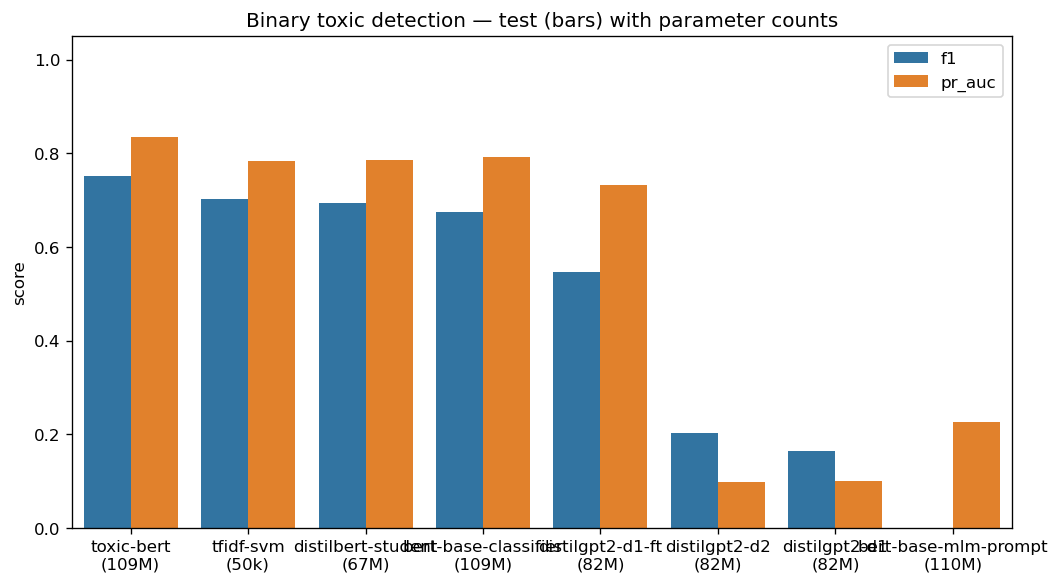
\includegraphics[width=\linewidth]{figures/model_comparison_bars_test.png}
%   \caption{Model comparison on test set.}
% \end{figure}

\textbf{Goal.} Establish a baseline comparison of all models on the same binary toxic task, and determine whether a larger model actually earns its cost.

\textbf{Protocol.} Score the val and test splits with each model's \texttt{predict\_toxic\_proba} at threshold~0.5. Measure F1, PR-AUC, ROC-AUC, and inference latency (ms/comment, CPU). Encoder and SVM use test $n{=}500$; decoder $n{=}200$.

\begin{table}[H]
\centering
\caption{Accuracy vs.\ efficiency (test set).}
\label{tab:accuracy}
\small
\begin{tabular}{@{}lrcccc@{}}
\toprule
\textbf{Model} & \textbf{Params} & \textbf{F1} & \textbf{PR-AUC} & \textbf{ROC-AUC} & \textbf{ms/comment} \\
\midrule
toxic-bert (BERT)       & 109M & 0.770 & 0.843          & 0.981 & 432   \\
tfidf-svm (non-neural)  & 50k  & 0.733 & \textbf{0.862} & 0.975 & \textbf{0.70} \\
distilgpt2-d2 (decoder) & 82M  & 0.206 & 0.102          & 0.45  & 769   \\
distilgpt2-d1 (decoder) & 82M  & 0.189 & 0.167          & 0.46  & 849   \\
\bottomrule
\end{tabular}
\end{table}

\textbf{Interpretation.} The linear model is close to toxic-bert on F1 and \textbf{beats its PR-AUC} at ${\sim}600\times$ lower latency---most of the task is lexical, confirming that raw accuracy alone does not justify a 109M-parameter transformer. The decoder is near chance (ROC-AUC $\approx 0.45$), consistent with H3: a small language model cannot discriminate toxicity without task-specific supervision.

\subsection{Fairness: Per-Identity FPR}\label{sec:fairness-results}

% \begin{figure}[t]\centering
%   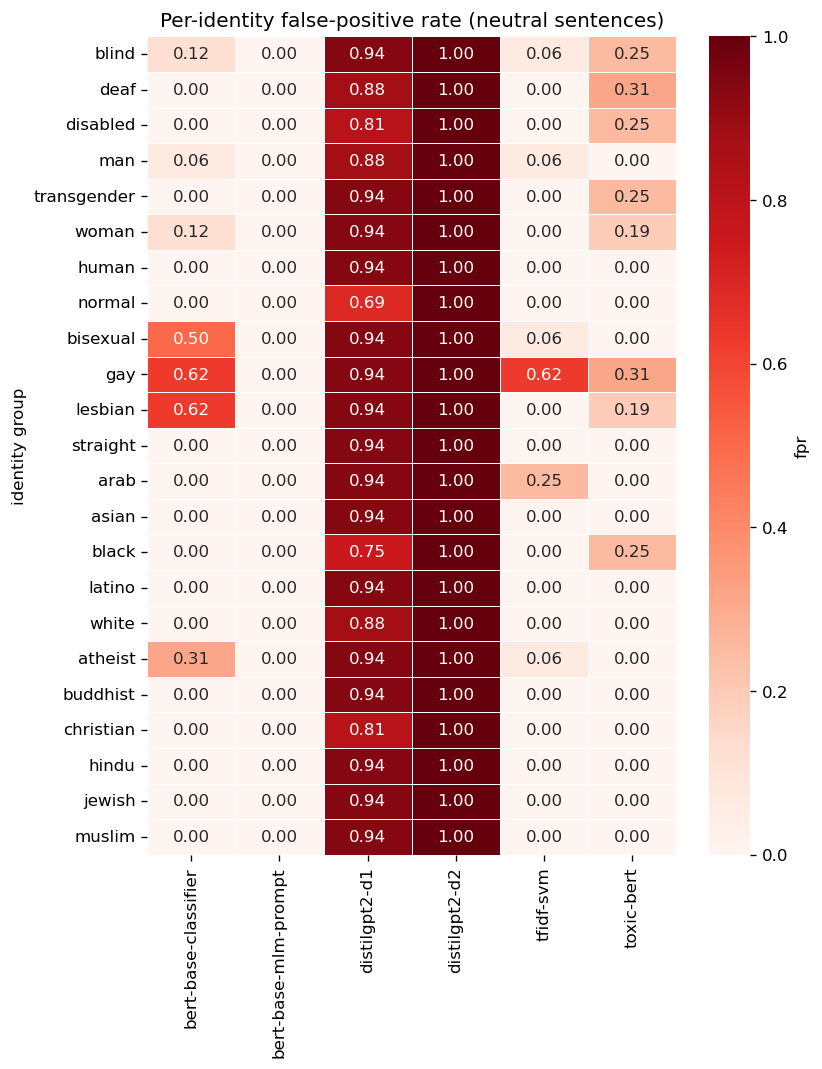
\includegraphics[width=\linewidth]{figures/fairness_fpr_heatmap.png}
%   \caption{Per-identity FPR heatmap.}
% \end{figure}

\textbf{Goal.} Test H1 (specialized encoder trades fairness for accuracy) by measuring how often each model wrongly flags neutral identity-mention sentences.

\textbf{Protocol.} Score the 210-sentence identity probe (\S\ref{sec:fairness}) plus 5 no-identity controls with each model at threshold~0.5. Report overall mean FPR across 21 groups and control FPR.

\begin{table}[H]
\centering
\caption{Identity FPR on neutral probe sentences.}
\label{tab:fairness}
\small
\begin{tabular}{@{}lcc@{}}
\toprule
\textbf{Model} & \textbf{Overall identity FPR} & \textbf{Control FPR} \\
\midrule
tfidf-svm        & 0.090 & 0.000 \\
toxic-bert       & 0.152 & 0.000 \\
distilgpt2-d1-ft & 0.505 & 0.000 \\
distilgpt2-d1    & 0.867 & \textbf{1.000} \\
\bottomrule
\end{tabular}
\end{table}

\textbf{Interpretation.} Control FPR is~0 for all trained classifiers, meaning false positives are \emph{specifically} identity-driven (``I am gay'', ``I am Muslim'' are flagged despite being non-toxic). The specialized encoder is \textbf{less fair} than the linear baseline (H1 supported). Zero-shot decoder flags essentially everything (control FPR~1.0); the D1 fine-tune removes that degeneracy (control~0) but still over-flags identity mentions (${\sim}$50\% FPR).

\subsection{Robustness to Obfuscation}

% \begin{figure}[t]\centering
%   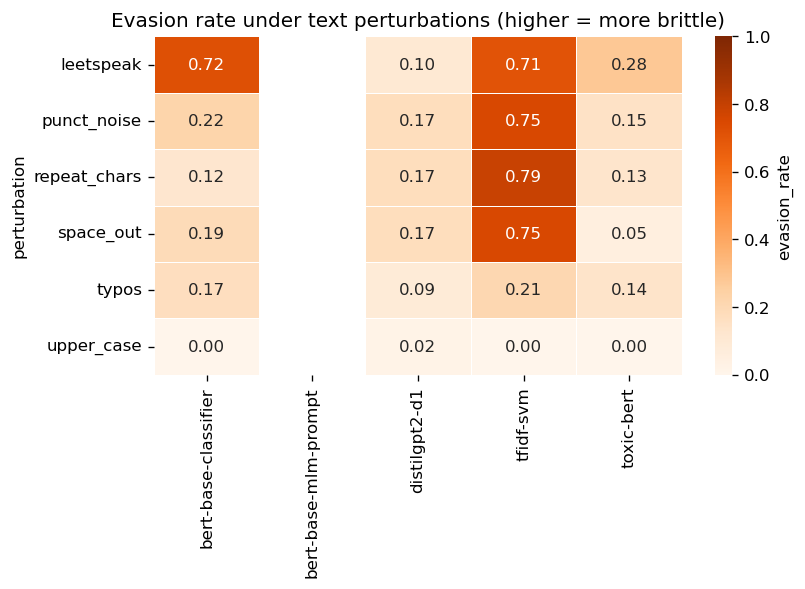
\includegraphics[width=\linewidth]{figures/robustness_evasion_heatmap.png}
%   \caption{Evasion rates by perturbation type.}
% \end{figure}

\textbf{Goal.} Determine which architecture is most resilient to the surface-level evasion tactics described in \S2.4.

\textbf{Protocol.} Take the subset of test comments that each model correctly flags as toxic (score $\ge 0.5$). Apply each perturbation and re-score. Report evasion rate.

\begin{table}[H]
\centering
\caption{Evasion rates (higher = more brittle).}
\label{tab:robustness}
\small
\begin{tabular}{@{}lcccc@{}}
\toprule
\textbf{Model} & \textbf{Baseline det.} & \textbf{Leetspeak} & \textbf{Space-out} & \textbf{Punct-noise} \\
\midrule
toxic-bert    & 0.92 & \textbf{0.28} & 0.03     & 0.15    \\
tfidf-svm     & 0.71 & 0.74          & 0.75     & 0.75    \\
distilgpt2-d1 & 0.58 & 0.10*         & 0.17*    & 0.17*   \\
\bottomrule
\end{tabular}
\end{table}

\textbf{Interpretation.} The encoder is far the most robust---its WordPiece tokenizer and contextual embeddings survive most surface noise. The SVM is trivially evaded because its TF-IDF features \emph{are} the surface tokens that perturbations destroy. The decoder's low evasion rate is misleading: its baseline detection is only~0.58 (near-random), so there is little left to evade. No model is fooled by upper-casing alone.

\subsection{Masking Intervention}

% \begin{figure}[t]\centering
%   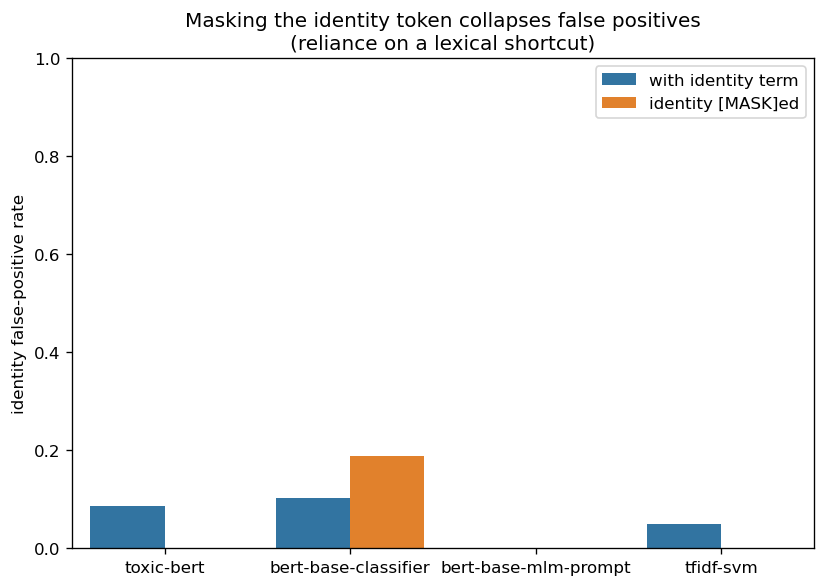
\includegraphics[width=0.48\linewidth]{figures/masking_inference_ablation.png}\hfill
%   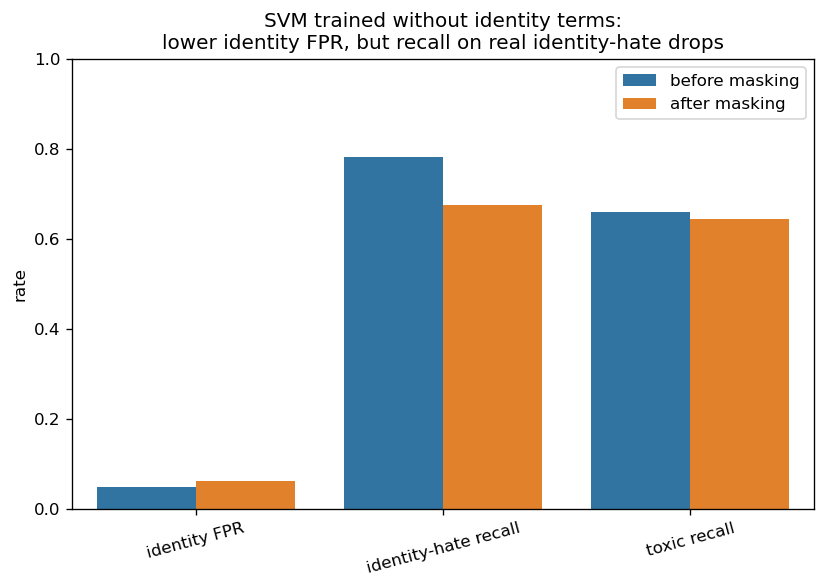
\includegraphics[width=0.48\linewidth]{figures/masking_svm_tradeoff.png}
%   \caption{Left: inference masking ablation. Right: SVM masking trade-off.}
% \end{figure}

\textbf{Goal.} Identify the \emph{mechanism} behind identity-term false positives (\S\ref{sec:fairness-results}): is the model relying on the identity token itself, or on surrounding context?

\textbf{Protocol.} (a)~\emph{Inference masking}: replace the identity term in each probe sentence with \texttt{[MASK]} (encoder) or empty string (SVM) and re-measure FPR. (b)~\emph{Training-time masking (SVM only)}: retrain on data with identity terms removed and compare identity FPR and identity-hate recall.

\textbf{Results.} Inference masking drops identity FPR from \textbf{0.152 to 0.000} (toxic-bert) and from \textbf{0.090 to 0.000} (SVM). Both architectures---a deep transformer and a bag-of-words---rely on the \textbf{identity token itself}: a lexical shortcut. Training-time masking of the SVM does \emph{not} reduce FPR ($0.090 \to 0.10$) but costs identity-hate recall ($0.78 \to 0.68$).

\textbf{Interpretation.} The bias is a single-token shortcut learned from the training data, not an architectural artifact. Naive token removal during training is an insufficient and harmful ``fix''---it sacrifices real identity-hate detection for negligible fairness improvement.

\subsection{Encoder vs.\ Decoder Agreement}

% \begin{figure}[t]\centering
%   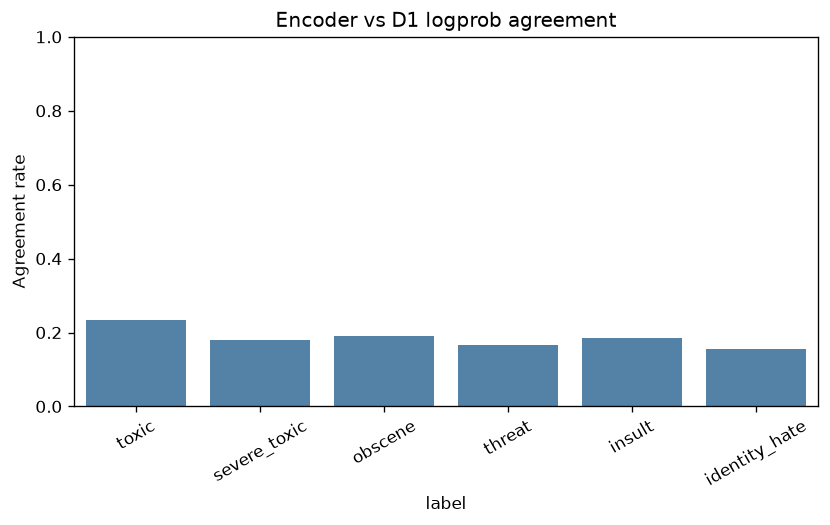
\includegraphics[width=0.48\linewidth]{figures/enc_dec_agreement.png}\hfill
%   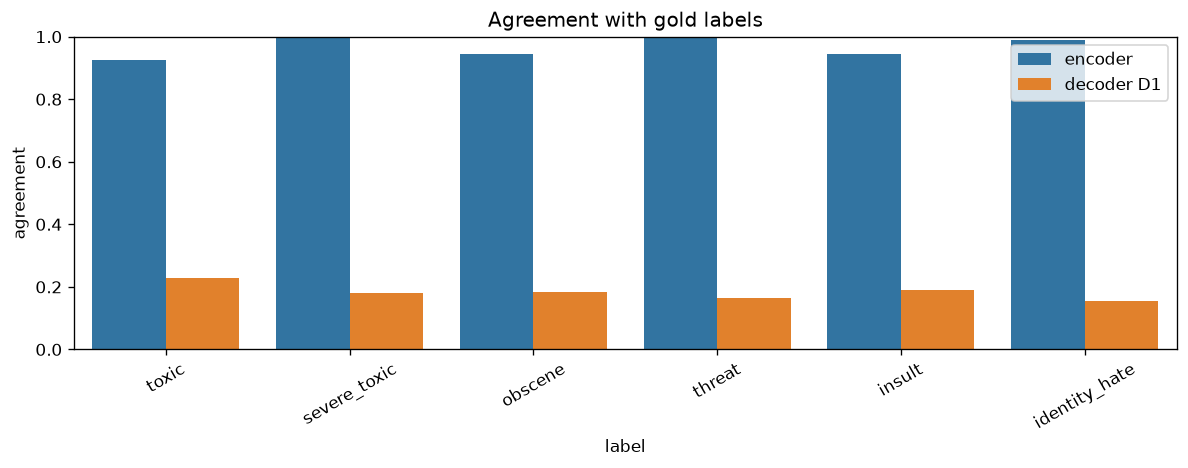
\includegraphics[width=0.48\linewidth]{figures/enc_dec_gold_agreement.png}
%   \caption{Left: encoder--decoder agreement. Right: each vs.\ gold.}
% \end{figure}

\textbf{Goal.} Measure how much the encoder and decoder agree, and whether disagreements reflect complementary signals or decoder degeneracy.

\textbf{Protocol.} Score 200 test comments with toxic-bert (6-label sigmoid) and DistilGPT-2 D1 (per-label yes/no prompt). For each label binarize at~0.5 and compute agreement rate, plus each model's agreement with gold.

\textbf{Results.} Overall encoder--decoder agreement is only \textbf{0.185}. Against gold on \texttt{toxic}, the encoder scores \textbf{0.925} but the decoder only \textbf{0.230}. Of 200 comments, the two disagree on \texttt{toxic} \textbf{153}~times---overwhelmingly decoder false positives on benign text:

\begin{table}[H]
\centering
\caption{Disagreement examples (test $n{=}200$).}
\label{tab:agreement}
\small
\begin{tabular}{@{}p{7.5cm}ccc@{}}
\toprule
\textbf{Comment (truncated)} & \textbf{Gold} & \textbf{Encoder} & \textbf{Decoder} \\
\midrule
``:Replied here:'' & 0 & 0 & 1 \\
``US New Citizenship Test. In October of 2008\ldots'' & 0 & 0 & 1 \\
``This is your last warning. You will be blocked\ldots'' & 0 & 0 & 1 \\
\bottomrule
\end{tabular}
\end{table}

\textbf{Interpretation.} Cross-architecture agreement is a poor proxy for correctness here. The disagreement stems from decoder degeneracy (labeling nearly everything toxic), not complementary insights. The encoder is right nearly every time.

\subsection{Distillation (Soft KD, 6 Labels)}

\textbf{Goal.} Test H2 (compression amplifies bias) by distilling toxic-bert into a smaller student and comparing accuracy and fairness.

\textbf{Protocol.} Train a 6-label DistilBERT student from frozen toxic-bert using soft KD ($T{=}2$, $\alpha{=}0.7$) + hard BCE. 20k train / 2k val, 4 epochs, best checkpoint by val macro-F1. Evaluate with the same binary harness and fairness probe.

\begin{table}[H]
\centering
\caption{Distillation: teacher vs.\ student.}
\label{tab:distill}
\small
\begin{tabular}{@{}lrcccl@{}}
\toprule
\textbf{Model} & \textbf{Params} & \textbf{Test F1} & \textbf{Identity FPR} & \textbf{ms/comment} & \textbf{Notes} \\
\midrule
toxic-bert (teacher)  & 109M & 0.770          & 0.152          & 274          & $n{=}500$ \\
distilbert-student    & 67M  & \textbf{0.772} & \textbf{0.062} & \textbf{159} & soft KD, 6-label \\
\bottomrule
\end{tabular}
\end{table}

\textbf{Interpretation (vs H2).} The student \textbf{matches} the teacher's toxic F1 (0.772 vs.\ 0.770) at ${\sim}1.7\times$ lower latency and \textbf{lower} overall identity FPR (0.062 vs.\ 0.152). Compression did \textbf{not} amplify identity bias---it reduced it. The likely mechanism: soft KD with temperature smoothing regularizes the student's confidence on identity-adjacent examples. Worst-group FPR remains concentrated (e.g.\ \texttt{gay}), suggesting the bias is not fully eliminated.

\subsection{Decoder Fine-Tune (D1 Yes/No, Binary Toxic)}

\textbf{Goal.} Determine whether the zero-shot decoder's failure (\S\ref{sec:accuracy}) is inherent to the architecture or simply a consequence of missing task supervision.

\textbf{Protocol.} Fine-tune DistilGPT-2 with causal LM loss \textbf{only on} the answer tokens (\texttt{yes}/\texttt{no}) after the same D1 prompt. 20k stratified train / 2k val, 4 epochs; best val answer accuracy \textbf{0.942}. Evaluate with the identical \texttt{score\_yes\_no} logprob path.

\begin{table}[H]
\centering
\caption{Decoder zero-shot vs.\ fine-tuned.}
\label{tab:decoder-ft}
\small
\begin{tabular}{@{}lcccl@{}}
\toprule
\textbf{Model} & \textbf{F1} & \textbf{ROC-AUC} & \textbf{Identity FPR} & \textbf{Notes} \\
\midrule
distilgpt2-d1 (zero-shot)  & 0.189          & 0.46           & 0.867 & degenerate \\
distilgpt2-d1-ft (fine-tuned) & \textbf{0.590} & \textbf{0.965} & 0.505 & usable ranking \\
\bottomrule
\end{tabular}
\end{table}

\textbf{Interpretation.} Light task-specific adaptation recovers strong discrimination (ROC-AUC $0.46 \to 0.97$; F1 $0.19 \to 0.59$) without changing architecture. This confirms that zero-shot failure reflects \emph{lack of supervision}, not architectural incapability. Identity FPR improves vs.\ zero-shot ($0.87 \to 0.51$; control FPR $1.0 \to 0.0$) but remains substantially worse than toxic-bert (0.15) and the SVM (0.09).

\subsection{On the Fairness of the Comparison}

A natural objection: is it fair to compare a \textbf{fine-tuned} encoder against a \textbf{zero-shot} decoder? Strictly speaking, the zero-shot decoder result (\S\ref{sec:accuracy}) measures \emph{deployment mode}, not architecture. We address this in several ways:

\begin{enumerate}[nosep]
  \item \textbf{The SVM is trained on the same data}---it is a genuinely fair baseline and nearly matches toxic-bert, showing that architecture alone does not explain the encoder's F1.
  \item \textbf{The D1 fine-tune (\S3.7)} gives the decoder the same type of supervision. Even with 20k examples, the fine-tuned decoder (F1~0.59) still trails the encoder (F1~0.77) and the SVM (F1~0.73)---a real gap that persists under controlled conditions.
  \item \textbf{The distillation student} is trained on the same data via KD and matches the teacher---a fair within-family comparison.
  \item \textbf{toxic-bert itself is favorable:} it was trained by Unitary on Jigsaw data, potentially with more data and tuning than we provide our own models. If anything, the comparison is biased \emph{toward} the encoder.
\end{enumerate}

We therefore frame the zero-shot decoder result as \emph{``what happens when you deploy an off-the-shelf LM without task adaptation''}---a practically important scenario---while the D1-ft result answers the architectural question more directly.

%----------------------------------------------------------------------
\section{Conclusions and Future Work}

\begin{enumerate}[nosep]
  \item \textbf{Toxicity detection is mostly lexical}---a 50k-feature linear model rivals a 109M encoder; ``bigger'' is not the story.
  \item \textbf{The encoder's real value is robustness to obfuscation}, not raw accuracy.
  \item \textbf{Zero-shot decoder prompting fails at DistilGPT-2 scale}---near chance and often degenerate; a \textbf{D1 fine-tune} (\S3.7) recovers usable discrimination (test F1~0.59, ROC-AUC~0.97) without changing architecture, though identity FPR stays high~(0.51).
  \item \textbf{Identity bias is data-driven, not architectural}---it appears even in the linear model, and masking the identity token erases it, revealing a lexical shortcut. Fixing it via naive training-masking trades recall for little gain.
  \item \textbf{Distillation (soft KD):} the DistilBERT student matches toxic-bert toxic F1 (0.772 vs.\ 0.770) at lower latency and \textbf{lower} identity FPR (0.062 vs.\ 0.152) on our probe---compression need not amplify bias (\textbf{H2} partially rejected).
\end{enumerate}

\textbf{Future work.} Soft-F1 regularization during distillation to directly optimize the evaluation metric; calibration analysis (ECE, reliability diagrams); larger evaluation samples for tighter confidence intervals; hateBERT cross-domain probe; neural masked fine-tune of DistilBERT as a debiasing intervention.

%----------------------------------------------------------------------
\section{References}

\begin{enumerate}[nosep,label={[\arabic*]}]
  \item Jigsaw/Conversation AI. Toxic Comment Classification Challenge. Kaggle, 2018.
  \item Dixon, Li, Sorensen, Thain, Vasserman. Measuring and Mitigating Unintended Bias in Text Classification. AIES 2018.
  \item Hanu, Unitary. Detoxify / \texttt{unitary/toxic-bert}, 2020.
  \item Sanh et al.\ DistilBERT, a distilled version of BERT: smaller, faster, cheaper and lighter. NeurIPS 2019 Workshop.
\end{enumerate}

%----------------------------------------------------------------------
\section{Ethics Statement (Required)}

\textbf{6.1 Introduction.} Names: Tom Jacob, Omer Ramon. Project title: \emph{Words That Harm}. In this project we aim to compare SVM, decoder-only, and encoder-only architectures for toxic-comment classification. We check for accuracy, identity bias, and robustness.

\textbf{6.2 Stakeholders and explanations.}
\begin{itemize}[nosep]
  \item \emph{Stakeholders:} (1)~platform users/commenters, (2)~human moderators, (3)~identity groups at risk of over-flagging.
  \item \emph{Explanations:} users need to know why a comment was flagged and how to appeal; moderators need per-label scores and confidence; identity groups need transparency about measured per-group false-positive rates.
  \item \emph{Responsibility:} the platform deploying the model owns user- and group-facing explanations; the ML team owns moderator-facing documentation.
\end{itemize}

\textbf{6.3 Our reflection (write ourselves---no LLM).}

\emph{[To be added by the team.]}

\end{document}
